\chapter{Introduction to File Systems}
\paragraph{}
Computers use secondary storage devices to permanently store data. To write the
data, a computer uses one of the widely known specifications. This allows the
computer to read back the data, once written. These specifications are more
commonly known by the term File Systems. File Systems enforce a uniform method
of storing and retrieving the data. Further, their popular nature allows the
device to be read properly across Operating Systems. You must have come across
at least a couple of file systems, if you have used a computer. Windows use NTFS
as its file system. Linux people prefer to use ext4 or btrfs. You USB drive most
probably uses the FAT32 file system.\\

So when you copy a file to your hard disk, you are writing to the file system
right? Actually, it is a bit more complicated than that. The computer does not
simply create a file system on top of your physical device. To create a file
system, you first need an abstraction, called a partition. Partition is a
logical slice of your physical device. It acts as a container onto which a file
system can be created. The partition maps to further abstracted versions of
physical locations on the drive. Suffice to say, a partition does not
necessarily have to occuppy the whole storage device. There can be more than one
partition and each partition can have different file systems, independant from
the rest of the partitions.\\

The process of creating partitions to store data on a storage device is called
disk partitioning. Apparently, ghosts of magnetic storage media are going to
haunt us for a very long time. You can read more about disk partitioning in the
next chapter.


\chapter{Disk Partitioning}
\paragraph{}
The term disk partitioning might bring up memories of slicing a pie. But let me
assure you that it is an entirely logical process. Disk partitioning makes a
secondary storage device usable. It creates partitions, which are then formatted
with a file system of our choice, and then used to store data. What if you just
want a single partition that spans an entire drive? You can ofcourse do that.
Still, the process you performed will be called partitioning.\\

It is very common to see systems with multiple partitions, and with a good
reason. Multiple partitions allow your system to be more flexible. There are
plethora of use cases for splitting up your disk, some of which are listed
below.

\begin{itemize}
    \item Separate personal information from Operating System files
    \item Separate boot information
    \item Run multiple operating systems
    \item Further partition personal data
    \item To have a faster partition for virtual memory
\end{itemize}

Never forget the fact that, each of these partitions are mere abstractions. They
are logical divisions which start from a sector of the drive and ends on an
other sector. If the partitions are purely logical, someone or something has to
keep track of their locations right? this is the job of the partition table.


\chapter{Partition table}
\paragraph{}
You have partitioned the device as per your heart's content. But as said before,
the partitions are purely logical creatures. They are abstractions. So where
does the computer store information on partitions? They cant be stored inside
the Operating System, as the data is needed first to understand where the OS is
stored. This is the job of the partition table. A partition table is usually
stored in the beginning of the drive. Every piece of low level software, that
tries to read data from the drive accesses the partition table first. Like the
plethora of file systems thriving in the wild, there are quite a few partition
table formats used by the leading platforms.

\section{Types}
Historically, the technology industry has taken great pride in keeping all the
knowledge they have gained to themselves. This meant new companies, trying to
bring some new product into the market often had to reinvent stuff that others
already had.\\

As a result, there are quite a few types of partition tables used by leading
platforms. Apple uses something called Apple Partition Map, BSD uses disklabel
but the most commonly used of them all is the Master Boot Record (MBR) and the
GUID (GPT) Partition Table.\\

If you are not the tinkering type and you own a decade old PC, your computer
most probably uses MBR. MBR started its life in the early 80s and carries with
it, all the limitations of the decade. It originally allowed only four
partitions (which was later fixed) and does not support drives of capacities
more than 2 TB. This lead Intel to develop a modern replacement called GPT. GPT
is the partition table used by most of the modern PCs. It has overcome most of
the limitations of the MBR.\\

So lets get this straight. You have the physical disk, on top of which, the
partition table exists. The partition table stores information on all those
imaginary partitions existing on the disk. The partitions are not physically
etched on the disk. This should mean they are pretty flexible right? Actually,
in reality, it is not that straight forward.

\begin{figure}
	\centering
	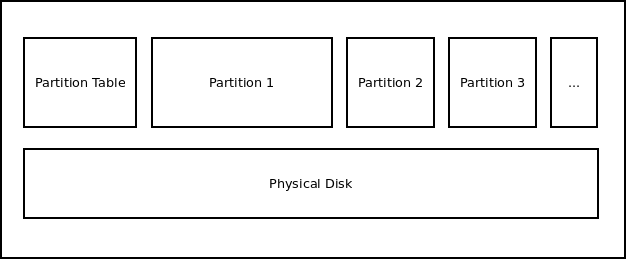
\includegraphics[scale=0.5]{partitions.png}
	\caption{Typical Partition table on a physical disk}
\end{figure}

\section{Disadvantages}
Let us imagine that we have a 500 GB Hard Disk, in which 465 GB is the actual
usable space (HDDs really do these nasty things). We split the drive into four
partitions as follows:

\begin{itemize}
    \item Partition 1 of size 50 GB for /
    \item Partition 2 of size 150 GB for /home
    \item Partition 3 of size 200 GB for Windows
    \item Partition 4 of size 65 GB for Backup
\end{itemize}

The drive is partitioned under the assumption that it will suffice for some time
. But within weeks, the / partition starts filling up. Your Windows partition
is virtually empty and you try to resize Windows so that you can get some space
for / partition except that you can't. The / partition can only acquire the
free space which is adjacent to it. And that by the way is the case with each
partition on the drive.\\

Further, if you want to modify the \ partition while the system is running, you
are out of luck. This is disastrous if you think of a production server which is
constantly serving the needs of clients. Most often, traditional partition
tables force you to boot into a live environment, if you want to modify anything
which the OS depends on.\\

Lets extend the production server concept bit further. Servers need lots of
space. If your firm is doing something worthwhile, space will eventually run out
and you will be forced to add more physical drives. Now you want the partition
having all your critical data to span across both the drives. There actually
exists a method called "Spanned Volume" on Windows which can do this but not
before destroying your current partition first. So yes, traditional partitioning
leaves you out in the cold when such situations arise. These are some of the
problems that gets fixed, when you switch to LVM.


\chapter{Logical Volume Manager}
\paragraph{}
If partitions are abtractions, Logical Volume Manager or LVM is an abstraction
on top of abstraction. So far we have talked about partitions, which are logical
structures on top of the physical disk. LVM extends this one step further by
creating logical volumes, which are usable partitions, on top of existing
partitions.\\

LVM is Linux's answer to all the problems discussed in the previous section, and
it can do a lot more. In LVM's lingo, the partitions on your drive is called
Physical Volume (PV). One or more physical volumes group together to form a
Volume Group (VG). A volume group appears as a single continuous space no matter
how many physical volumes lie underneath. LVM works by creating partitions
called Logical Volumes (LV) on top of the volume group.\\

By virtue of definition, the logical volumes can span across physical drives,
also they bring a number of goodies to the table, the most prominent being the
ability to resize partitions on the fly. This means, switching into a live
environment or even unmounting the partition is no longer necessary.

\begin{figure}
	\centering
	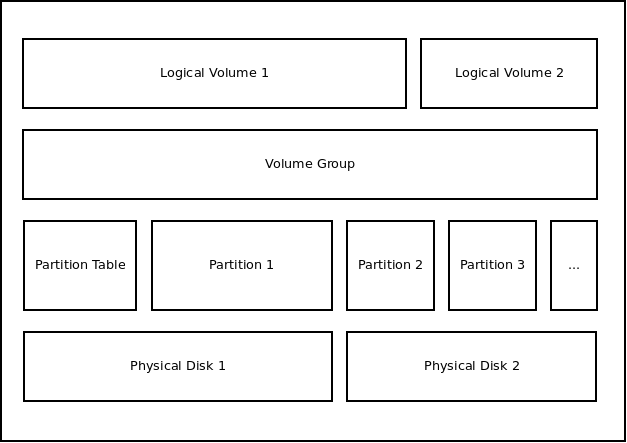
\includegraphics[scale=0.5]{lvm.png}
	\caption{Typical LVM structure}
\end{figure}


\section{Implementation}
The high level, logical nature of LVM means Linux cannot access it like the
traditional partitions. To solve the issue, Linux uses a piece of code called
Device Mapper. Device Mapper passes data from a virtual device such as a logical
volume to the physical storage device. The snapshot functionality, about which
you will read in the next section is implemented by the device mapper. The use
of device mapper extends beyond implementing the LVM. It can be used for
encrypting disks and simulating hardware behaviour.

\section{Snapshots}
Disks fail. Operating Systems crashes. Viruses can attack. All of these can take
your precious data with them. Backing up data is an option, but what if you want
to save the current state of your storage? This is where disk imaging comes into
play. Disk imaging allows the creation of image of your entire disk. Normally,
this is done by rebooting your computer and booting into a live environment such
as CloneZilla. Which means, you guessed it, more downtime.\\

LVM provides a very handy feature called snapshots, which are like disk images,
except that you can create one while your system is up. Snapshots allows you to
create images of your entire storage which can be used to restore disks to the
state at the time of creation of the snapshot. The advantage is obvious. You can
continue to server your clients or do your work, while LVM creates a copy of
your entire drive for future use. Once created, these images act like logical
volumes, which can be mounted if required.

\section{Striped Volume}
Lets imagine you have two independant physical drives, which are capable of
operating, well, independantly. That means, while one drive is doing its job,
the one is free to do something else. Enter striped volume.\\

Striped volumes are logical volumes, that can span more than one physical drive.
The advantage is obvious. You will reading and writing at twice the speed of
a single drive. There are alternatives to this, such as using RAID. But LVM
shines through due to ease of setting up the system.

\section{Advantages}
\begin{itemize}
    \item Ability to resize partition without shutting down or even unmounting
    \item A single partition can span one or more physical drives
    \item Take snapshot of entire storage while the system is up
    \item Striped volumes that can provide enhanced performance
\end{itemize}

\section{Disadvantages}
\begin{itemize}
    \item LVM is Linux only and is not supported under Windows
    \item If a physical drive fails while using striped volume, data can be lost
    \item LVM cannot offer raw disk performance
\end{itemize}


\chapter{RAID}
\paragraph{}
RAID stands for Redundant Array of Inexpensive (or Independant) Disks depending
on whom you ask. RAID is a method for combining disk drives for increasing
performance, reliability or both. RAID can operate differently according to mode
in which it operates. There are seven standard modes numbered from 0 to 7. We
are not going to discuss all of them as it exceeds the scope of this report.
RAID provides a number of features that are similar to the ones provided by LVM,
but differences exist, which are discussed in this chapter.

\section{RAID Striping}
Except RAID 1, all RAID levels support the creation of striped partitions. If
RAID is implemented through a dedicated hardware card, the striping is
transparent to the Operating System and as a side effect, performs considerably
faster than an LVM striped volume.\\

When you create a striped volume, the main concern is the reliability of the
drives working underneath. If a drive fails, it can make the data inaccessible
or useless. RAID level 5 and up tackles this issue by using distributed parity.
In simpler words, data correction mechanisms make sure that the data stays
accesible even if one of the drives in the array fails. But the technology is
not without its faults.

\section{Disadvantages}
First of all, RAID striping requires that all of the drives be of same capacity.
If the computer initially had a 500 GB drive and you bought an additional 1 TB
drive to do striping, congrats. Now you have two drives with the usable size of
500 GB. In other words, the extra 500 GB of your new HDD cannot be used. The
usable size of each drive in a RAID array implementing striping is the size of
the drive having the least size. So if your computer initially had a 500 GB
drive, you have to keep buying drives of the capacity 500 GB or throw out the
older drive. I call that expensive.\\


